\documentclass[a4paper,12pt]{article}
	
\usepackage[T2A]{fontenc}			
\usepackage[utf8]{inputenc}			
\usepackage[english,russian]{babel}	

\usepackage[
bookmarks=true, colorlinks=true, unicode=true,
urlcolor=black,linkcolor=black, anchorcolor=black,
citecolor=black, menucolor=black, filecolor=black,
]{hyperref}

\usepackage{color}
\usepackage{caption}


\usepackage{amsmath,amsfonts,amssymb,amsthm,mathtools} 
\usepackage{wasysym}

\usepackage{graphicx}
%\usepackage[cache=false]{minted}
\usepackage{cmap}
\usepackage{indentfirst}

\usepackage{listings} 
\usepackage{fancyvrb}
\usepackage{slashbox}

\usepackage{geometry}
\geometry{left=2cm}
\geometry{right=1.5cm}
\geometry{top=1cm}
\geometry{bottom=2cm}

\setlength{\parindent}{5ex}
\setlength{\parskip}{0.5em}

\usepackage{titlesec}
\usepackage{pgfplots}
\usepackage{filecontents}
\usetikzlibrary{datavisualization}
\usetikzlibrary{datavisualization.formats.functions}

\DeclareCaptionFont{white}{\color{white}}
\DeclareCaptionFormat{listing}{\colorbox{gray}{\parbox{\textwidth}{#1#2#3}}}
\captionsetup[lstlisting]{format=listing,labelfont=white,textfont=white}
\lstloadlanguages{% Check Dokumentation for further languages ...
C,
C++,
csh,
Java
}

\definecolor{red}{rgb}{0.6,0,0} % for strings
\definecolor{blue}{rgb}{0,0,0.6}
\definecolor{green}{rgb}{0,0.8,0}
\definecolor{cyan}{rgb}{0.0,0.6,0.6}

\lstset{ %
language=Lisp,                 % выбор языка для подсветки
basicstyle=\small\sffamily, % размер и начертание шрифта для подсветки кода
numbers=left,               % где поставить нумерацию строк (слева\справа)
numberstyle=\tiny,           % размер шрифта для номеров строк
stepnumber=1,                   % размер шага между двумя номерами строк
numbersep=5pt,                % как далеко отстоят номера строк от подсвечиваемого кода
showspaces=false,
backgroundcolor=\color{white},         
showstringspaces=false,      % показывать или нет пробелы в строках
showtabs=false,             % показывать или нет табуляцию в строках
frame=single,              % рисовать рамку вокруг кода
tabsize=2,                 % размер табуляции по умолчанию равен 2 пробелам
captionpos=t,              % позиция заголовка вверху [t] или внизу [b] 
breaklines=true,           % автоматически переносить строки (да\нет)
breakatwhitespace=false, % переносить строки только если есть пробел
escapeinside={\%*}{*)}
}

% Для измененных титулов глав:
\definecolor{gray75}{gray}{0.75} % определяем цвет
\newcommand{\hsp}{\hspace{20pt}} % длина линии в 20pt
% titleformat определяет стиль
\titleformat{\chapter}[hang]{\Huge\bfseries}{\thechapter\hsp\textcolor{gray75}{|}\hsp}{0pt}{\Huge\bfseries}

\begin{document}
	
\begin{figure}[h!]
	\begin{center}
		{
\includegraphics[width = \textwidth]{titul.png}}
	\end{center}
\end{figure}

\vspace*{20mm}

\huge
\begin{center}
	Лабораторная работа №6
\end{center}


\vspace*{50mm}

\large
\begin{flushleft}
	Студент: Луговой Д.М. \\
	Группа: ИУ7-61Б \\
	Преподаватель: Толпинская Н.Б.
\end{flushleft}

\vspace*{60mm}

\large
\begin{center}
	Москва, 2020 г.
\end{center}

\thispagestyle{empty}

\newpage
\vspace*{10mm}
\textbf{Цель работы}: приобрести навыки работы в Common Lisp.\\

\textbf{Задачи работы}: изучить работу интерпретатора Lisp, алгоритм работы функции eval, структуру и порядок обработки программы в Lisp.

\begin{enumerate}
\item \textbf{Способы определения функций}

Новые функции можно определить с помощью оператора defun. Он принимает три или более аргументов: имя, список параметров и ноль или более выражений, которые составляют тело функции. 

(defun func\_name (arg1 arg2 ... argN) func\_body)

Но функция не обязательно должна иметь имя, для того, чтобы определить функцию, не имеющую имени, необходимо воспользоваться лямбда-выражением. Лямбда-выражение – это список, содержащий символ lambda и следующие за ним список аргументов и тело, состоящее из нуля или более выражений.

(lambda (arg1 arg2 .. argN) func\_body)

\item \textbf{Вызовы функций, блокировка их выполнения}

Для простейшего вызова функции используется список, первый элемент которого трактуется как имя функции, а остальные - как ее аргументы. Любое введенное S-выражение передается функции EVAL, которая вычисляет его и возвращает результат его вычисления. Схема работы функции EVAL:
\begin{figure}[ht!]
\center{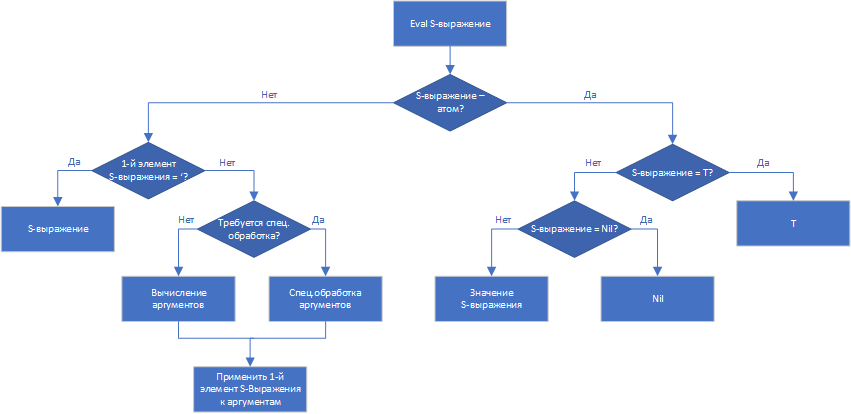
\includegraphics[scale=0.82]{FaLP1.png}}
\end{figure}

\newpage
\vspace*{10mm}
Для явного вызова функции в Lisp используются функционалы APPLY и FUNCALL. APPLY принимает первым аргументом функцию, а вторым - список аргументов, которые будут переданы в функцию. FUNCALL принимает переменное число аргументов, первый из которых функция, а остальные - аргументы, которые будут переданы в функцию. Оба функционала возвращают результаты вычисления переданной им функции при переденной ей аргументах.

Для того, чтобы заблокировать вычисление S-выражения используется функция QUOTE, или ее обозначение '. Она принимает S-выражение и возвращает его же, таким образом блокируя его вычисление.

\item \textbf{Локальное и глобальное определение значения атома}

Локальные значение атома можно определить с помощью функций let и let*. Областью видимости является тело функции, в которой определена переменная.

Синтаксис:

(let ((var1 value1) (var2 value2) ... (varN valueN)) body)

Сначала вычисляются значения value1, value2, ... , valueN, а затем происходит их связывание с var1, var2, ... , varN. 

(let* ((var1 value1) (var2 value2) ... (varN valueN)) body)

Отличие от let состоит в том, что связывание каждого значения value с символом var происходит сразу после вычисления значения.

Глобальные значение атома устанавливается с помощью функции setf. Областью видимости является весь код, следующий после определения.

Синтаксис: 

(setf var value)
\end{enumerate}
\newpage
\vspace*{10mm}
{\LARGE Задание №1}\\

Переписать функцию how-alike, приведенную в лекции и использующую COND, использую конструкции IF, AND/OR.

\begin{lstlisting}[caption=Переписанная функция how-alike]
(defun how-alike (x y) (if (or (= x y)(equal x y)) 'the_same
	(if (and (oddp x)(oddp y)) 'both_odd
		(if (and (evenp x)(evenp y)) 'both_even
			 'difference
			)
		)
	)
)
\end{lstlisting}

Пример:
\begin{lstlisting}
> (how_alike 1 1)
THE_SAME
> (how_alike 1 6)
DIFFERENCE
> (how_alike 8 4)
BOTH_EVEN
> (how_alike 5 7)
BOTH_ODD
\end{lstlisting}

{\LARGE Задание №2}\\

Даны 2 списка: с названиями стран и с названиями столиц.

Написать функции для создания:
\begin{itemize}
\item списка из двухэлементых списков, содержащих страну и столицу;
\item списка из точечных пар, содержащих страну и столицу.
\end{itemize}

\begin{lstlisting}[caption=Функция создания списка из двухэлементных списков]
(defun join_in_lists (countries capitals) (mapcar #'(
	lambda 
		(country capital)
		(cons country 
			(cons capital nil)
		)
	) 
	countries capitals
))
\end{lstlisting}

\newpage
\vspace*{10mm}

Пример:
\begin{lstlisting}
> (join_in_lists '(Russia England USA Ukraine) '(Moscow London Washington Kiev))
((RUSSIA MOSCOW) (ENGLAND LONDON) (USA WASHINGTON) (UKRAINE KIEV))
\end{lstlisting}

\begin{lstlisting}[caption=Функция создания списка из точечных пар]
(defun join_in_pairs (countries capitals)(mapcar #'cons countries capitals))
\end{lstlisting}

Пример:
\begin{lstlisting}
> (join_in_pairs '(Russia England USA Ukraine) '(Moscow London Washington Kiev))
((RUSSIA . MOSCOW) (ENGLAND . LONDON) (USA . WASHINGTON) (UKRAINE . KIEV))
\end{lstlisting}

Написать функции для поиска страны по столице и столицы по стране.

\begin{lstlisting}[caption=Функция поиска в списке двухэлементных списков]
(defun find_in_lists_list (name lst) (cond 
	((OR
		(car 
			(rassoc (cons name nil) lst :test 'equal)
		)
		(cadr
			(assoc name lst)
		)
	))
))
\end{lstlisting}
Пример:

\begin{lstlisting}
> (setf lists (join_in_lists '(Russia England USA Ukraine) '(Moscow London Washington Kiev))
((RUSSIA MOSCOW) (ENGLAND LONDON) (USA WASHINGTON) (UKRAINE KIEV))
> (find_in_lists_list 'London lists)
ENGLAND
> (find_in_lists_list 'USA lists)
WASHINGTON
> (find_in_lists_list 'Paris lists)
NIL
\end{lstlisting}

\newpage
\vspace*{10mm}

\begin{lstlisting}[caption=Функция поиска в списке точечных пар]
(defun find_in_pairs_list (name lst) (cond 
	((OR
		(car 
			(rassoc name lst)
		)
		(cdr
			(assoc name lst)
		)
	))
))
\end{lstlisting}

Пример:
\begin{lstlisting}
> (setf pairs (join_in_pairs '(Russia England USA Ukraine) '(Moscow London Washington Kiev)))
((RUSSIA . MOSCOW) (ENGLAND . LONDON) (USA . WASHINGTON) (UKRAINE . KIEV))
> (find_in_pairs_list 'Kiev pairs)
UKRAINE
> (find_in_pairs_list 'Russia pairs)
MOSCOW
> (find_in_pairs_list 'India pairs)
NIL
\end{lstlisting}

\end{document}